
\newpage
{\bfseries IRSTI 20.20.20}

{\bfseries OPTIMAL CONTROL OF AN UNMANNED AERIAL VEHICLE}

{\bfseries \textsuperscript{1}A.T. Mazakova, \textsuperscript{1}Т Sh.A.
Jomartova, \textsuperscript{1,2}T.Zh. Mazakov\textsuperscript{🖂}, G.Ch.
\textsuperscript{3}Т Toikenov,}

{\bfseries \textsuperscript{2}M.S. Aliaskar}

¹Kazakh National University named after Al-Farabi, Almaty, Kazakhstan,

²International Engineering and Technology University, Almaty,
Kazakhstan,

³Kazakh National Women\textquotesingle s Pedagogical University, Almaty,
Kazakhstan

{\bfseries \textsuperscript{🖂}}Corresponding author: tmazakov@mail.ru

The main objective of this work is to develop algorithms and software
solutions for finding optimal control strategies for an unmanned aerial
vehicle, the mathematical model of which is represented by a system of
ordinary differential equations. Using the maximum principle, an
algorithm was developed to determine the optimal control. The presented
methods and models are of high practical importance for managing various
economic and technical systems.

{\bfseries Key words}: UAV, dynamics, mathematical model, controllability,
stability.

{\bfseries ҰШҚЫШСЫЗ ҰШУ АППАРАТЫН ОҢТАЙЛЫ БАСҚАРУ}

{\bfseries \textsuperscript{1}А.Т. Мазақова,
\textsuperscript{1}Ш.А.Джомартова, \textsuperscript{1,2}Т.Ж.
Мазаков\textsuperscript{🖂}, \textsuperscript{3}Г.Ч. Тойкенов,}

{\bfseries \textsuperscript{2}М.С. Әлиаскар}

\textsuperscript{1}Әл-Фараби атындағы Қазақ ұлттық университеті, Алматы,
Қазақстан,

\textsuperscript{2}Халықаралық инженерлік-технологиялық университеті,
Алматы, Қазақстан,

\textsuperscript{3}Қазақ ұлттық қыздар педагогикалық университеті,
Алматы, Қазақстан,

е-mail: tmazakov@mail.ru

Бұл жұмыстың негізгі міндеті-математикалық моделі қарапайым
дифференциалдық теңдеулер жүйесімен ұсынылған дронды басқарудың оңтайлы
стратегияларын іздеу үшін алгоритмдер мен бағдарламалық шешімдерді құру.
Максимум принципін қолдана отырып, оңтайлы басқаруды анықтау үшін
алгоритм жасалды. Ұсынылған әдістер мен модельдер әртүрлі экономикалық
және техникалық жүйелерді басқарудың жоғары практикалық маңыздылығына
ие.

{\bfseries Түйін сөздер:} ҰҰА, динамика, математикалық модель,
басқарылғыштық, тұрақтылық.

{\bfseries ОПТИМАЛЬНОЕ УПРАВЛЕНИЕ БЕСПИЛОТНЫМ ЛЕТАТЕЛЬНЫМ АППАРАТОМ}

{\bfseries \textsuperscript{1}А.Т. Мазакова,
\textsuperscript{1}Ш.А.Джомартова, \textsuperscript{1,2}Т.Ж.
Мазаков\textsuperscript{🖂}, \textsuperscript{3}Тойкенов Г.Ч.,}

{\bfseries \textsuperscript{2}М.С. Алиаскар}

\textsuperscript{1}Казахский национальный университет имени аль-Фараби,
Алматы, Казахстан,

\textsuperscript{2}Международный инженерно-технологический университет,
Алматы, Казахстан,

\textsuperscript{3}Казахский национальный женский педагогический
университет, Алматы, Казахстан,

е-mail: tmazakov@mail.ru

Главная задача данной работы заключается в создании алгоритмов и
программных решений для поиска оптимальных стратегий управления
беспилотным летательным аппаратом, чья математическая модель
представлена системой обыкновенных дифференциальных уравнений. Используя
принцип максимума, был разработан алгоритм для определения оптимального
управления. Представленные методы и модели обладают высокой практической
значимостью для управления различными экономическими и техническими
системами.

{\bfseries Ключевые слова}: БПЛА, динамика, математическая модель,
управляемость, устойчивость.

{\bfseries Introduction.} Unmanned aviation is actively developing
worldwide due to the growing demand for lightweight, relatively
inexpensive aircraft with high maneuverability, capable of performing a
wide range of tasks. Unmanned aerial vehicles (UAVs) are successfully
used in both military operations and civilian applications, including
linearization {[}1-5{]}.

The study of many aviation systems is reduced to the creation of
mathematical models described by nonlinear ordinary differential
equations. However, no universal solution methods have been developed
for nonlinear systems. It is important to consider the nature of
nonlinearities when studying such mathematical models.

Optimization of control is one of the key tasks in the theory of
controlled dynamic systems. To design and operate aviation systems, it
is necessary to achieve the goal with maximum efficiency, which requires
minimizing a certain quality functional.

{\bfseries Materials and Methods.} The work is devoted to the study of
optimal control of the mathematical model of UAV dynamics:

\begin{longtable}[]{@{}
  >{\raggedright\arraybackslash}p{(\columnwidth - 2\tabcolsep) * \real{0.9470}}
  >{\raggedright\arraybackslash}p{(\columnwidth - 2\tabcolsep) * \real{0.0530}}@{}}
\toprule\noalign{}
\begin{minipage}[b]{\linewidth}\raggedright
\[\left\{ \begin{matrix}
\dot{V} = g(n_{xa} - sin\Theta) \\
\dot{\Theta} = g(n_{ya}cos\gamma - cos\Theta)/V \\
\begin{matrix}
\dot{\Psi} = - gn_{ya}sin\gamma/(Vcos\Theta) \\
\dot{x} = Vcos\Theta\cos\Psi \\
\begin{matrix}
\dot{y} = Vsin\Theta \\
\dot{z} = - Vcos\Theta\sin\Psi
\end{matrix}
\end{matrix}
\end{matrix} \right.\ \]
\end{minipage} & \begin{minipage}[b]{\linewidth}\raggedright
(1)
\end{minipage} \\
\midrule\noalign{}
\endhead
\bottomrule\noalign{}
\endlastfoot
\end{longtable}

\begin{longtable}[]{@{}
  >{\raggedright\arraybackslash}p{(\columnwidth - 2\tabcolsep) * \real{0.9470}}
  >{\raggedright\arraybackslash}p{(\columnwidth - 2\tabcolsep) * \real{0.0530}}@{}}
\toprule\noalign{}
\begin{minipage}[b]{\linewidth}\raggedright
\[n_{xa} = \frac{Pcos\alpha - X_{a}}{mg},\ n_{ya} = \frac{Psin\alpha + Y_{a}}{mg}\]
\end{minipage} & \begin{minipage}[b]{\linewidth}\raggedright
(2)
\end{minipage} \\
\midrule\noalign{}
\endhead
\bottomrule\noalign{}
\endlastfoot
\end{longtable}

Where:

\begin{itemize}
\item
  \emph{x, y, z} are the coordinates of the aircraft\textquotesingle s
  center of mass in the normal Earth coordinate system;
\item
  \emph{V} is the flight speed;
\item
  \emph{ϴ} is the trajectory angle;
\item
  \emph{Ψ} is the course angle;
\item
  \emph{α} is the angle of attack;
\item
  \emph{γ} is the roll angle;
\item
  \emph{P} is the engine thrust;
\item
  \(X_{a}\) is aerodynamic drag;
\item
  \(Y_{a}\) is aerodynamic lift;
\item
  \emph{m} is the mass of the aircraft;
\item
  \emph{g} is gravitational acceleration;
\item
  \(n_{xa}\) is the longitudinal overload;
\item
  \(n_{ya}\) is the lateral overload (in flow axes of coordinates)
  {[}6-7{]}.
\end{itemize}

Overloads \(n_{xa}\), \(n_{ya}\) and the roll angle \emph{γ} are taken
as control variables in (1).

We introduce the following notation:

\begin{longtable}[]{@{}
  >{\raggedright\arraybackslash}p{(\columnwidth - 2\tabcolsep) * \real{0.9470}}
  >{\raggedright\arraybackslash}p{(\columnwidth - 2\tabcolsep) * \real{0.0530}}@{}}
\toprule\noalign{}
\begin{minipage}[b]{\linewidth}\raggedright
\[q = \begin{bmatrix}
V \\
\Theta \\
\begin{matrix}
\Psi \\
x \\
\begin{matrix}
y \\
z
\end{matrix}
\end{matrix}
\end{bmatrix},\ q_{0} = \begin{bmatrix}
V_{0} \\
\Theta_{0} \\
\begin{matrix}
\Psi_{0} \\
x_{0} \\
\begin{matrix}
y_{0} \\
z_{0}
\end{matrix}
\end{matrix}
\end{bmatrix},\ q_{1} = \begin{bmatrix}
V_{1} \\
\Theta_{1} \\
\begin{matrix}
\Psi_{1} \\
x_{1} \\
\begin{matrix}
y_{1} \\
z_{1}
\end{matrix}
\end{matrix}
\end{bmatrix}\]
\end{minipage} & \begin{minipage}[b]{\linewidth}\raggedright
(3)
\end{minipage} \\
\midrule\noalign{}
\endhead
\bottomrule\noalign{}
\endlastfoot
\end{longtable}

The system of equations (1) is rewritten as the following system of
nonlinear ordinary differential equations:

\begin{longtable}[]{@{}
  >{\raggedright\arraybackslash}p{(\columnwidth - 2\tabcolsep) * \real{0.9483}}
  >{\raggedright\arraybackslash}p{(\columnwidth - 2\tabcolsep) * \real{0.0517}}@{}}
\toprule\noalign{}
\begin{minipage}[b]{\linewidth}\raggedright
\(\dot{\mathbf{x}}\mathbf{= f}\left( \mathbf{x,t} \right)\mathbf{+ Bu(t)}\).
\end{minipage} & \begin{minipage}[b]{\linewidth}\raggedright
(4)
\end{minipage} \\
\midrule\noalign{}
\endhead
\bottomrule\noalign{}
\endlastfoot
\end{longtable}

Where:

\begin{itemize}
\item
  \emph{f(x,t)} is an n-vector whose elements are continuously
  differentiable functions of their arguments;
\item
  x is an n-dimensional system state vector;
\item
  u is scalar control.
\end{itemize}

Control is subject to constraints:

\begin{longtable}[]{@{}
  >{\raggedright\arraybackslash}p{(\columnwidth - 2\tabcolsep) * \real{0.9470}}
  >{\raggedright\arraybackslash}p{(\columnwidth - 2\tabcolsep) * \real{0.0530}}@{}}
\toprule\noalign{}
\begin{minipage}[b]{\linewidth}\raggedright
\[u(t) \in U = \left\{ u(t):\ u(t) \in C\lbrack\left\lbrack t_{0},t_{1} \right\rbrack; - L \leq u(t) \leq L,\ t \in \left\lbrack t_{0},t_{1} \right\rbrack \right\}.\]
\end{minipage} & \begin{minipage}[b]{\linewidth}\raggedright
(5)
\end{minipage} \\
\midrule\noalign{}
\endhead
\bottomrule\noalign{}
\endlastfoot
\end{longtable}

The problem is to find a control satisfying constraint (5) that
transfers the system from the initial state

\begin{longtable}[]{@{}
  >{\raggedright\arraybackslash}p{(\columnwidth - 2\tabcolsep) * \real{0.9470}}
  >{\raggedright\arraybackslash}p{(\columnwidth - 2\tabcolsep) * \real{0.0530}}@{}}
\toprule\noalign{}
\begin{minipage}[b]{\linewidth}\raggedright
\(x\left( t_{0} \right) = x_{0}\).
\end{minipage} & \begin{minipage}[b]{\linewidth}\raggedright
(6)
\end{minipage} \\
\midrule\noalign{}
\endhead
\bottomrule\noalign{}
\endlastfoot
\end{longtable}

to the final specified state

\begin{longtable}[]{@{}
  >{\raggedright\arraybackslash}p{(\columnwidth - 2\tabcolsep) * \real{0.9470}}
  >{\raggedright\arraybackslash}p{(\columnwidth - 2\tabcolsep) * \real{0.0530}}@{}}
\toprule\noalign{}
\begin{minipage}[b]{\linewidth}\raggedright
\(x\left( t_{1} \right) = x_{1}\).
\end{minipage} & \begin{minipage}[b]{\linewidth}\raggedright
(7)
\end{minipage} \\
\midrule\noalign{}
\endhead
\bottomrule\noalign{}
\endlastfoot
\end{longtable}

within a fixed time \(t_{1} - t_{0}\).

For the quality assessment of system performance, the following criteria
can be selected:

\begin{longtable}[]{@{}
  >{\raggedright\arraybackslash}p{(\columnwidth - 2\tabcolsep) * \real{0.9463}}
  >{\raggedright\arraybackslash}p{(\columnwidth - 2\tabcolsep) * \real{0.0537}}@{}}
\toprule\noalign{}
\begin{minipage}[b]{\linewidth}\raggedright
\[J = \int_{t_{0}}^{T}{\left\lbrack u^{*}(t)R_{0}u(t) \right\rbrack dt}\]
\end{minipage} & \begin{minipage}[b]{\linewidth}\raggedright
(8)
\end{minipage} \\
\midrule\noalign{}
\endhead
\bottomrule\noalign{}
\endlastfoot
\end{longtable}

In functional (8), \(R_{0}\) is a positively definite \emph{m}х\emph{m}
matrix. The required state at the final time can be specified as fixed
(7) or changing (satisfying certain conditions).

\begin{longtable}[]{@{}
  >{\raggedright\arraybackslash}p{(\columnwidth - 2\tabcolsep) * \real{0.9463}}
  >{\raggedright\arraybackslash}p{(\columnwidth - 2\tabcolsep) * \real{0.0537}}@{}}
\toprule\noalign{}
\begin{minipage}[b]{\linewidth}\raggedright
\[\sum_{j = 1}^{n}c_{ij}x_{j}(T) \leq d_{i},i = \overline{1,k}\]
\end{minipage} & \begin{minipage}[b]{\linewidth}\raggedright
(9)
\end{minipage} \\
\midrule\noalign{}
\endhead
\bottomrule\noalign{}
\endlastfoot
\end{longtable}

The optimal control problem is considered, including control constraints
(5) with fixed (7) or variable boundaries (8). Currently, solving such
problems is accompanied by many mathematical difficulties. Various
formulations of optimal control problems will be considered. The task is
to minimize the functional (8) under the constraints (4), (5), (6), and
(7). The time moment \(T\) is considered given (fixed).

To solve the optimal control problem, we will construct the Hamilton
function:

\begin{longtable}[]{@{}
  >{\raggedright\arraybackslash}p{(\columnwidth - 2\tabcolsep) * \real{0.9333}}
  >{\raggedright\arraybackslash}p{(\columnwidth - 2\tabcolsep) * \real{0.0667}}@{}}
\toprule\noalign{}
\begin{minipage}[b]{\linewidth}\raggedright
\(H\left( x(t),u,\psi(t),\psi_{0} \right) = u^{*}(t)R_{0}u(t) + (g(x,t) + Bu(t))^{*}\psi_{}\).
\end{minipage} & \begin{minipage}[b]{\linewidth}\raggedright
(10)
\end{minipage} \\
\midrule\noalign{}
\endhead
\bottomrule\noalign{}
\endlastfoot
\end{longtable}

And form the conjugate system of differential equations:

\begin{longtable}[]{@{}
  >{\raggedright\arraybackslash}p{(\columnwidth - 2\tabcolsep) * \real{0.9343}}
  >{\raggedright\arraybackslash}p{(\columnwidth - 2\tabcolsep) * \real{0.0657}}@{}}
\toprule\noalign{}
\begin{minipage}[b]{\linewidth}\raggedright
\[\frac{d\psi}{dt} = - (\frac{\partial g(t)}{\partial t})^{*}(t)\psi(t),\ t \in \left\lbrack t_{0}, ⥂ \mspace{6mu} T \right\rbrack.\]
\end{minipage} & \begin{minipage}[b]{\linewidth}\raggedright
(11)
\end{minipage} \\
\midrule\noalign{}
\endhead
\bottomrule\noalign{}
\endlastfoot
\end{longtable}

The optimal control is determined by condition (5) and the maximum of
the Hamiltonian:

\begin{longtable}[]{@{}
  >{\raggedright\arraybackslash}p{(\columnwidth - 2\tabcolsep) * \real{0.9333}}
  >{\raggedright\arraybackslash}p{(\columnwidth - 2\tabcolsep) * \real{0.0667}}@{}}
\toprule\noalign{}
\begin{minipage}[b]{\linewidth}\raggedright
\[u = \left\{ \begin{matrix}
0 & если & R_{0}^{- 1}B\psi < 0 \\
R_{0}^{- 1}B\psi & если & 0 \leq R_{0}^{- 1}B\psi \leq u_{\max} \\
u_{\max} & если & R_{0}^{- 1}B\psi > u_{\max}\{
\end{matrix} \right.\ \]
\end{minipage} & \begin{minipage}[b]{\linewidth}\raggedright
(12)
\end{minipage} \\
\midrule\noalign{}
\endhead
\bottomrule\noalign{}
\endlastfoot
\end{longtable}

\emph{Theorem:} Let the pair
\(\left( u(t),x(t) \right),\ t \in \lbrack t_{0}, ⥂ \mspace{6mu} T\rbrack\)
be the solution to the problem posed above. Then, there necessarily
exists a vector function
\(\psi(t),t \in \lbrack t_{0}, ⥂ \mspace{6mu} T\rbrack\) and a parameter
\begin{figure}[H]
	\centering
	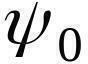
\includegraphics[width=0.8\textwidth]{assets/149}
	\caption*{}
\end{figure} such that:

1) \(\psi_{0} \leq 0\),
\(\left| \psi_{0} \right| + \left| \psi(t) \right| \neq 0,\ t \in \lbrack t_{0}, ⥂ \mspace{6mu} T\rbrack\)

2) The pair
\(x(t),\psi(t),\quad t \in \lbrack t_{0}, ⥂ \mspace{6mu} T\rbrack\) is
the solution to the boundary value problem for the system of
differential equations (4) and the corresponding conjugate system of
differential equations (11) with boundary conditions (6) and (7) and
control (12).

Next, we study the problem of optimal control with fixed boundaries
(6)-(7) and control constraints (5). Currently, solving such problems
also encounters certain mathematical difficulties.

For the practical solution of the control optimization problem, penalty
function methods and the gradient method are applied. To account for
constraints at the end of the trajectory (7), we introduce a penalty
function
\(Ф_{k} = М_{k}\sum_{i = 1}^{n}\left\lbrack x(T) - x_{T}) \right\rbrack^{2}\),
where \(\{ М_{k}\}\) is a predefined positive sequence tending to
infinity. We construct a new functional:

\begin{figure}[H]
	\centering
	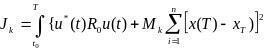
\includegraphics[width=0.8\textwidth]{assets/150}
	\caption*{}
\end{figure}

The problem can be reformulated as follows: for a given value of the
parameter \emph{k}, find the optimal control minimizing the functional
\(J_{k}\)\hspace{0pt} subject to constraints (5)-(7). This problem
belongs to the class of optimal control problems with a free right
boundary and control constraints.

For it, we will construct the Hamiltonian function:

\[H_{k} = u^{*}(t)R_{0}u(t) + (g(x,t) + Bu(t))^{*}\psi_{k}\]

The following solution algorithm is proposed:

Step 1: Let \(k = 0\) .

Step 2: Calculate the optimal control for the k-th iteration using
equation (12), where \(ᴪ_{k}\) is the solution to the conjugate system
of differential equations (11), with the boundary condition at the end:

\begin{longtable}[]{@{}
  >{\raggedright\arraybackslash}p{(\columnwidth - 2\tabcolsep) * \real{0.9333}}
  >{\raggedright\arraybackslash}p{(\columnwidth - 2\tabcolsep) * \real{0.0667}}@{}}
\toprule\noalign{}
\begin{minipage}[b]{\linewidth}\raggedright
\[\Psi_{k}(T) = 2M_{k}\sum_{i = 1}^{n}{\lbrack x_{k}(T) - x_{T}\rbrack}\]
\end{minipage} & \begin{minipage}[b]{\linewidth}\raggedright
(13)
\end{minipage} \\
\midrule\noalign{}
\endhead
\bottomrule\noalign{}
\endlastfoot
\end{longtable}

and \(x_{k}\) is the solution of the original system (4) with initial
conditions (6).

Step 3: Calculate the value of the functional \(J_{k}\) for the obtained
\(x_{k}\) and \(u_{k}\).

Step 4: If \(\left| J_{k} - J_{k - 1} \right| \leq \varepsilon\) proceed
to step 5, otherwise, set \(k = k + 1\) and go back to step 2. (Here,
\(\varepsilon > 0\) is the required accuracy of the calculation).

Step 5: The found pair (\(x_{k}\), \(u_{k}\)) is the optimal solution.

To automate the process of finding the optimal control, a program
"Optim\_Upr.m" was written in MATLAB. As a result of its execution, we
obtain the analytical form of the original and conjugate systems of
differential equations, the form of the Hamiltonian function for the UAV
mathematical model (1)-(3):

H=10.*ux\^{}2+10.*uy\^{}2+(9.80*ux-9.80*sin(O))*fi1+(5.15*uy-9.80*cos(O))/V*fi2-8.34*uy/V/cos(O)*fi3+V*cos(O)*cos(K)*fi4+V*sin(O)*fi5-1.*V*cos(O)*sin(K)*fi6

f1=9.80*ux-9.80*sin(O)

f2=(5.15*uy-9.80*cos(O))/V

f3=-8.34*uy/V/cos(O)

f4=V*cos(O)*cos(K)

f5=V*sin(O)

f6=-1.*V*cos(O)*sin(K)

fp1=(5.15*uy-9.80*cos(O))/V\^{}2*fi2-8.34*uy/V\^{}2/cos(O)*fi3-1.*cos(O)*cos(K)*fi4-1.*sin(O)*fi5+cos(O)*sin(K)*fi6

fp2=9.80*cos(O)*fi1-9.80*sin(O)/V*fi2+8.34*uy/V/cos(O)\^{}2*fi3*sin(O)+V*sin(O)*cos(K)*fi4-1.*V*cos(O)*fi5-1.*V*sin(O)*sin(K)*fi6

fp3=V*cos(O)*sin(K)*fi4+V*cos(O)*cos(K)*fi6

fp4=0

fp5=0

fp6=0

H1=-20.*ux-9.80*fi1

H2=-20.*uy-5.15/V*fi2+8.34/V/cos(O)*fi3

Here f1,\ldots,f6 is the view of the right side of the initial system of
differential equations, fp1,\ldots,fp6 is the view of the right side of
the conjugate system.

The obtained results are transferred to a program written in Delphi,
which performs numerical calculations to find the optimal control.

The results of the program are output to the file "rez.txt," a fragment
of which is provided below:

T=1,00 nt=1000

-10,00\textless=U1\textless=10,00

-5,00\textless=U2\textless=5,00

x0 = 8,00; = 1,00; = 3,00; = 5,00; = 1,00; = 3,00;

xk = 4,00; = 0,50; = 1,50; = 2,50; = 0,50; = 1,50;

F1 == 1009,53 11276,69 11276,69

F2 == 1164,04 20148,99 10102,31

F3 == 1191,48 40409,25 10874,49

F4 == 1127,07 42853,26 5356,66

F5 == 1250,00 184817,12 4551,07

F6 == 1244,47 321606,47 3050,20

A total of 6 functionals F1,\ldots,F6. were calculated. As can be seen
from the last column, the difference between the specified and final
points decreases.

{\bfseries Results and Discussion}. Constructing the conjugate system of
differential equations (11) for the original nonlinear system (1) is a
rather labor-intensive process, especially when the dimensionality
\emph{n} increases, and is practically impossible for \emph{n}
\textgreater{} 3. Furthermore, when forming the Hamiltonian function,
there is often a "human factor" involved, which does not guarantee the
correctness of the analytical calculations. Therefore, the automation of
verifying the conditions of the theorems becomes relevant.

To address this issue, it is recommended to use computer algebra systems
(CAS), such as MATLAB {[}8-9{]}. These systems provide a wide range of
tools for working with algebraic expressions, from simple operations
like calculation and differentiation to more complex ones like series
expansion and integration. The application of such systems is relevant
in various industries, including the aerospace industry.

Numerical calculations showed correspondence with experimental data. The
results are also saved in text files, allowing the visualization of UAV
dynamics in the form of one-dimensional graphs using MATLAB, for which a
special program was developed. Based on the presented theory, an
application was created {[}10{]}.

{\bfseries Conclusions.} The development of unmanned aviation requires the
creation of optimal control methods for dynamic systems, which is
crucial for enhancing the efficiency of unmanned aerial vehicle (UAV)
management. This study confirms the necessity of finding optimal
solutions in the presence of nonlinear equations and control
constraints.

The article proposes a mathematical model of UAV dynamics described by a
system of nonlinear differential equations. Several variants of the
optimal control problem were solved with fixed and variable boundaries,
as well as by using penalty functions and the gradient method to find
optimal trajectories. The solution to the optimal control problem
involves minimizing a functional under given constraints, which requires
significant mathematical computations.

The application of a computer algebra system (MATLAB) enabled the
automation of complex differential equation system calculations and
minimized the human factor, which is important for increasing the
accuracy of computations. Numerical calculations confirmed the
correctness of the proposed theoretical model. The results showed
consistency between calculated data and real experimental observations,
indicating the applicability of the model for real UAV control systems.

The developed "Optim\_Upr.m" program in MATLAB, along with the
application created for visualizing the results, simplifies solving UAV
dynamics control tasks and provides results in the form of text files
and graphs. This opens up opportunities for the further application of
these methods in real-world conditions.

The continued use and development of the proposed algorithms and
software can significantly improve the efficiency of UAV control
systems, enabling them to adapt to changing real-time conditions and be
applied in various industries, including the aviation and space sectors.

\emph{{\bfseries Financing:} The The work was carried out with the support
of the Research Institute of Mathematics and Mechanics at Al-Farabi
Kazakh National University and grant funding for scientific research for
2023--2025 under project AP19678157.}

{\bfseries References}

1.Loginov A.A., Hvan A.A. Aktual\textquotesingle nost\textquotesingle{}
ispol\textquotesingle zovanija bespilotnyh letatel\textquotesingle nyh
apparatov// Aktual\textquotesingle nye problemy aviacii i kosmonavtiki.
-- 2015.-T.1.- S.704 -705.{[}in Russ.{]}

2. Husnutdinov T.D., Shherbakova A.V., Komarova P.A., Rublevskaja E.V.,
Reshetnikov A.Ju. Perspektivy ispol\textquotesingle zovanija bespilotnyh
letatel\textquotesingle nyh apparatov v innovacionnyh proektah//
Aktual\textquotesingle nye problemy aviacii i kosmonavtiki.- 2017.-
T.3.- S.139-141. {[}in Russ.{]}

3.Lju Sh., Li., Tan C., Vu Sh., God\textquotesingle e Zh.-L. Razrabotka
bespilotnyh transportnyh sredstv.- M.:DMK Press.- 2022.-246 s. ISBN
978-5-97060-969-9. {[}in Russ.{]}

4.Avgustov L.I i dr. Navigacija letatel\textquotesingle nyh apparatov v
okolozemnom prostranstve. -- M.: OOO «Nauchtehlitizdat», 2015. -592s.
ISBN 978-5-93728-146-3. {[}in Russ.{]}

5.Berns V.A., Dolgopolov A.V. i dr. Jeksperimental\textquotesingle nyj
modal\textquotesingle nyj analiz letatel\textquotesingle nyh apparatov.
-- Novosibirsk: NGTU, 2023. -- 328 s. ISBN 978-5-7782-3209-9{[}in
Russ.{]}

6.Tang Than\textquotesingle{} Lam Sistemnyj analiz i optimizacija
rezhimov poleta dlja upravlenija letatel\textquotesingle nym apparatom
// Avtoref. disser. kand. tehn. nauk, spec. 05.13.01, Moskva, 2015. --
155 s. {[}in Russ.{]}

7. Mazakova A., Jomartova Sh.,Vfzakov T., Shormanov., Amirkhanov B.
Controllability of an unmanned aerial vehicle.// 2022 IEEE 7th
International Energy Conference (ENERGYCON) - C.1-5.
DOI~10.1109/ENERGYCON53164.2022.9830244

8.Smolencev N.K. MatLAb. Programmirovanie na Visual C\#, Borland
JBuilder, VBA. -- M.: DMK Press, 2009. -- 464s.

9.D\textquotesingle jakonov V., Abramenkova I. MATLAB. Obrabotka
signalov i izobrazhenij. Special\textquotesingle nyj spravochnik. --
SPb.: Piter, 2002. - 608 s. ISBN 5-318-00667-1.

10. A.C. № 45572 ot 05.10.2024. Mazakova A.T., Dzhomartova S.A., Mazakov
T.Ja. Opredelenie optimal\textquotesingle nogo upravlenija BPLA.
Komp\textquotesingle juternaja programma

\emph{{\bfseries Information about the authors}}

Mazakova A.T. - PhD student of the Al-Farabi Kazakh National University,
Almaty, Kazakhstan, e-mail: aigerym97@mail.ru;

Jomartova Sh.A. - Doctor of Technical Sciences, Associate Professor,
Al-Farabi Kazakh National University, Almaty, Kazakhstan, e-mail:
jomartova@mail.ru;

Mazakov T.Zh. -- Doctor of Physical and mathematical sciences,
professor, Al-Farabi Kazakh National University, Almaty, Kazakhstan,
e-mail: tmazakov@mail.ru;

Tokenov G.Ch. - Candidate of Physical and Mathematical Sciences,
Associate Professor, Kazakh National Women\textquotesingle s Pedagogical
University, Almaty, Kazakhstan, e-mail: gumyrbektoike@mail.ru;

Aliaskar M.S. - Lecturer at the International University of Engineering
and Technology, Almaty, Kazakhstan, e-mail: m.alyasqar@gmail.ru

\emph{{\bfseries Сведение об авторах}}

Мазақова А.Т. -- докторант Казахского национального университета
им.аль-Фараби, e-mail: aigerym97@mail.ru;

Джомартова Ш.А. - доктор технических наук, доцент, Казахский
национальный университет им. аль-Фараби, Алматы, Казахстан, e-mail:
jomartova@mail.ru;

Мазаков Т.Ж. -- доктор физико-математических наук, профессор, Казахский
национальный университетим. аль-Фараби, Алматы, Казахстан, e-mail:
tmazakov@mail.ru;

Тойкенов Г.Ч. - кандидат физико-математических наук, доцент, Казахский
национальный женский педагогический университет, Алматы, Казахстан,
e-mail: gumyrbektoike@mail.ru;

Әлиасқар М.С. - докторант Казахского национального университета
им.аль-Фараби, Алматы, Казахстан, e-mail: m.alyasqar@gmail.ru

